\section{Topología básica en $\mathbb{R}$}

\begin{definicion}
	Sea $X$ un conjunto no vacío. Una familia de subconjuntos $\tau$ de $X$ es una topología sobre $X$ si: 
	\begin{enumerate}
		\item $\Phi, X, \in \tau$. 
		\item Cualquier familia $\{A_i\}$ de elementos de $\tau$ es tal que $\cup_i A_i\in\tau$. 
		\item Si $A_1,A_2\in \tau \implies A_1\cap A_2 \in \tau$. 
	\end{enumerate}
\begin{nota}
	A los elementos de $\tau$ se les llama abiertos de $X$. 
\end{nota}
\end{definicion}

\begin{definicion}
	La familia $\theta$ de todos los subconjuntos abiertos de $M$ es la topología de $M$ y el par $(M, \theta)$ es el espacio topológico asociado al métrico $M$.
	\begin{nota}
		En el caso de $\mathbb{R}^n$ se dice que se tiene el espacio topológico Euclidiano $\mathbb{R}^n$. 
	\end{nota}
\end{definicion}

\begin{ejemplo}
	\begin{enumerate}
		\item $\mathbb{R}^n$ es abierto. En efecto, $B_1(x)\subset \mathbb{R}^n, \forall x\in\mathbb{R}^n$. 
		\item $G=\{x\in\mathbb{R}:0<x<1\}$ es abierto,  pero $F=\{x\in\mathbb{R}:0\leq x<1\}$ no lo es. 
	\end{enumerate}

\begin{center}
	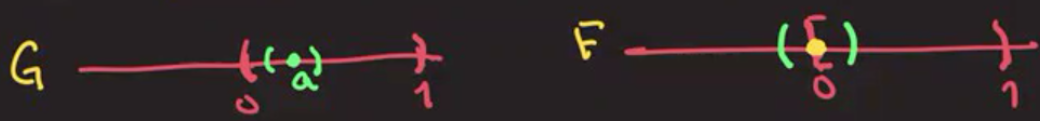
\includegraphics[scale=0.4]{images/2/1}
\end{center}
\end{ejemplo}

\begin{ejemplo}
	\begin{enumerate}
		\item $G=\{(x,y)\in\mathbb{R}^2\ni x^2+y^2<1\}$ es abierto. 
		\item $F=\{(x,y)\in \mathbb{R}^2\ni x^2+y^2\leq 1\}$ no es abierto. 
	\end{enumerate}
\begin{center}
	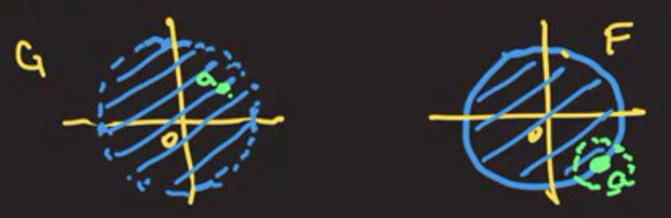
\includegraphics[scale=0.4]{images/2/2}
\end{center}
\end{ejemplo}

\begin{ejemplo}
	\begin{enumerate}
		\item $G=\{(x,y)\in\mathbb{R}^2\ni 0<x<1, y=0\}$ no es abierto de $\mathbb{R}^2$. 
		\item $F=\{(x,y)\in \mathbb{R}^2\ni 0<x<1\}$ es abierto de $\mathbb{R}^2$. 
	\end{enumerate}
	\begin{center}
		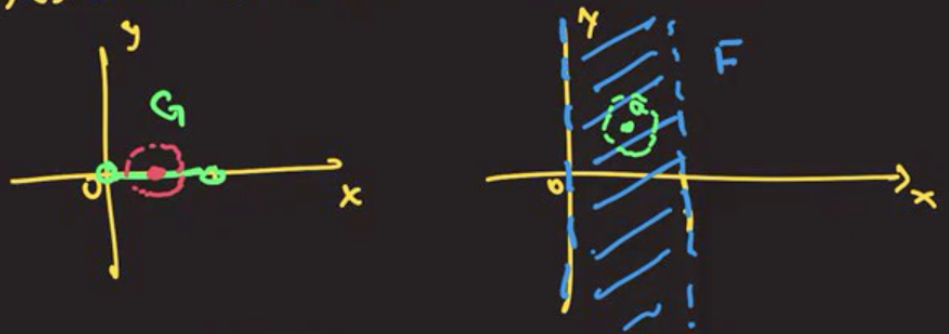
\includegraphics[scale=0.4]{images/2/3}
	\end{center}
\end{ejemplo}
\begin{ejemplo}
	$\Phi$ es abierto.
\end{ejemplo}

\begin{prop}
	Una bola abierta es abierto. 
\end{prop}
\begin{proof}
	Sea $x\in B_r(a)$ y considere la bola centrada en $x$ y de radio $r-d(a,x)$. A probar: $B_{r-d(a,x)}(x)\subset B_r(a)$. Sea $y\in B_{r-d(a,x)}(x)$. Entonces, 
	\begin{align*}
		d(a,y) &\leq d(a,x)+d(x,y)\\
		&< d(a,x)+[r-d(a,x)]\\
		&= r
	\end{align*}
$\implies y \in B_r(a)$. 

 	\begin{center}
 	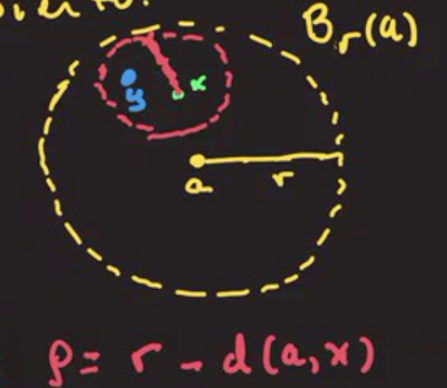
\includegraphics[scale=0.4]{images/2/4}
 \end{center}
\end{proof}

\begin{teorema}
	Considere $(\mathbb{R}^n,d)$: 
	\begin{enumerate}
		\item $\Phi$ y $\mathbb{R}^n$ son abiertos. 
		\item La intersección de dos abiertos de $\mathbb{R}^n$ es abierto de $\mathbb{R}^n$. 
		\begin{cajita}
			Por inducción, se deduce que la intersección finita de abiertos es abierto. 
		\end{cajita}
		\item La unión de cualquier colección de abiertos es un abierto de $\mathbb{R}^n$. 
	\end{enumerate}
\end{teorema}

\begin{proof}
	\item OK. 
	\item Sea $A$ y $B$ abiertos de $\mathbb{R}^n$. A probar: $A\cap B$ es abierto. Sea $x\in A\cap B$, entonces: 
	\begin{enumerate}
		\item $x\in A$, abierto, $\implies \ \exists r>0\ni d(x,z)<r$, para $z\in A$. 
		\item $x\in B$, abierto, $\implies \ \exists r'>0\ni d(x,w)<r$, para $w\in B$.  
	\end{enumerate}
	\begin{center}
	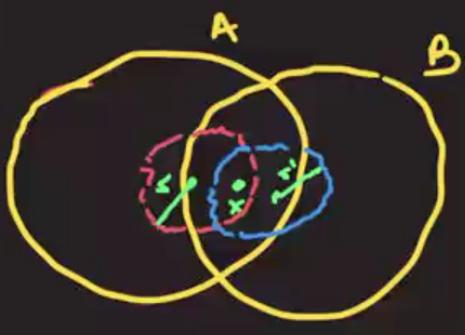
\includegraphics[scale=0.4]{images/2/5}
\end{center}
	$\implies$ Hagamos $r=\min\{r,r'\}\implies $ si $y\in \mathbb{R}\ni d(x,y)<r\implies y\in A$ y $y\in B\implies y\in A\cap B\implies A\cap B$ es abierto en $\mathbb{R}^n$. 
	
	\item Sea $\{G_\alpha\}$ una colección cualquiera de abierto de $\mathbb{R}^n$, y sea $G=\cup_{\alpha} G_\alpha$. Si $x\in G\implies x\in G_\lambda$, para algún $\lambda$. Como $G_\lambda$ es abierto $\implies \ \exists r>0 \ni B_r(x)\subset G_\lambda \subset \cup_\alpha G_\alpha =G$. 
\end{proof}

\begin{nota}
	La intersección de una colección infinita de abierto no necesariamente es abierto. En efecto considere: 
	\begin{align*}
		A_n &= \{x\in\mathbb{R}\ni -\frac{1}{n}<x<1+\frac{1}{n}\}, \quad n\in\mathbb{Z}^+\\
		A_1 &= (-1,2)\\
		A_2 &= \left(-\frac{1}{2}, \frac{3}{2}\right)\\
		&\vdots\\
		\implies A &= \cap_{n=1}^\infty A_n\\
	&= [0,1]\quad \text{¿Por qué cerrado?}
		\end{align*}
	
	\begin{cajita}
		Los $A_n$ son abiertos (por se bolas abiertas de $\mathbb{R}$)
	\end{cajita}
\end{nota}

\begin{definicion}
	Un subconjunto $\mathbb{F}$ en el métrico $(M,d)$ es cerrado si $\mathbb{F}^c$ es abierto. 
\end{definicion}
\begin{center}
	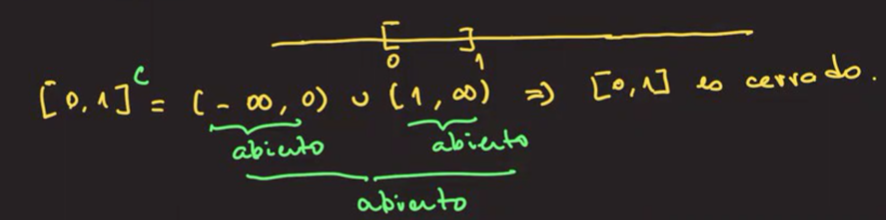
\includegraphics[scale=0.4]{images/2/6}
\end{center}

\begin{cajita}
	\begin{enumerate}
		\item Abierto: bola abierta contenida en $A$ es cada punto. 
		\begin{center}
			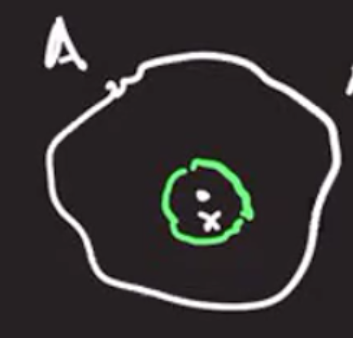
\includegraphics[scale=0.3]{images/2/7}
		\end{center}
	\item Topología (colección de todos los abiertos) en el métrico. 
	\item $F$ es cerrado si $F^c$ es abierto. 
	\item Abierto y cerrado no son negación uno del otro. \begin{enumerate}
		\item $\Phi$, $\mathbb{R}^n$ son abiertos y cerrados. 
		\item $[0,1)$ no es abierto ni cerrado. 
	\end{enumerate}
	\end{enumerate}
\end{cajita}

\begin{definicion}
	Sea $x\in M$ (espacio métrico), entonces cualquier conjunto que contiene un abierto $A\ni x\in A$ es una vecindad de $x$. 
\end{definicion}

\begin{ejemplo}
	Sea
	\begin{center}
		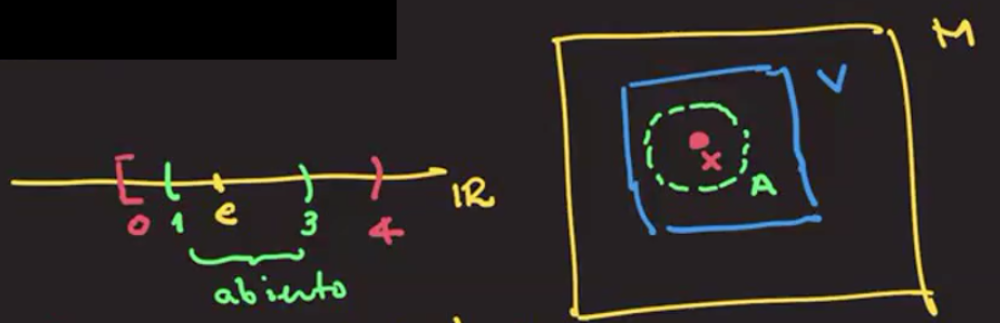
\includegraphics[scale=0.4]{images/2/8}
	\end{center}
\begin{enumerate}
	\item $[0,4)$ es na vecindad de $e$. 
	\item $(1,3)$ es vecindad abierta de $e$. 
	\item $\mathbb{R}$ es vecindad de $e$. 
	\item $(e-\varepsilon, e+\varepsilon)$ es vecindad de $e, \ \forall \varepsilon >0$. 
\end{enumerate}
\end{ejemplo}

\begin{definicion}
	Un punto $x\in M$ es punto interior de un conjunto $A\subseteq M$, si $A$ es una vecindad de $M$. 
	\begin{enumerate}
		\item $[0,1]$, $x=0$ y $x=1$; no son puntos interiores. El resto de punto $(0,1)$ son puntos interiores de $[0,1]$. 
		\item En $I=(0,1)$, todos son puntos interiores. 
		\item $\mathbb{R}\cap \mathbb{Z}\subseteq \mathbb{R}$. 
		\begin{center}
			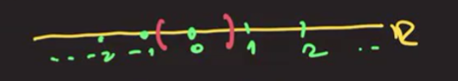
\includegraphics[scale=0.4]{images/2/9}
		\end{center}
	$\implies \mathbb{R}\cap \mathbb{Z}$ no tiene puntos interiores.  
	\end{enumerate}
\end{definicion}

\begin{definicion}
	Un punto $x$ es un punto de acumulación (o punto límite) de un conjunto $A\subseteq M$, si cada vecindad de $x$ contiene al menos un punto de $A$ diferente de $x$. Es decir, si 
	$$(B_r(x)-\{x\})\cap A\neq \emptyset, \quad \forall r>0.$$
\end{definicion}

\begin{ejemplo}
	$A=\{1,1/2,1/3,\cdots, 1/n, \cdots \}\subseteq \mathbb{R}\implies x=0$ es un punto de acumulación de $A$. 
	\begin{center}
		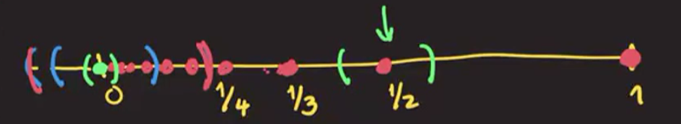
\includegraphics[scale=0.4]{images/2/10}
	\end{center}
\end{ejemplo}
	\begin{center}
	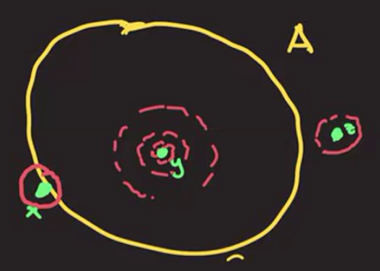
\includegraphics[scale=0.4]{images/2/11}
\end{center}

\begin{definicion}
	El conjunto de todos los puntos interiores de $A$ se llama interior de $A$ (Notación: $A^\circ$ o $int(A)$). 
	\begin{center}
		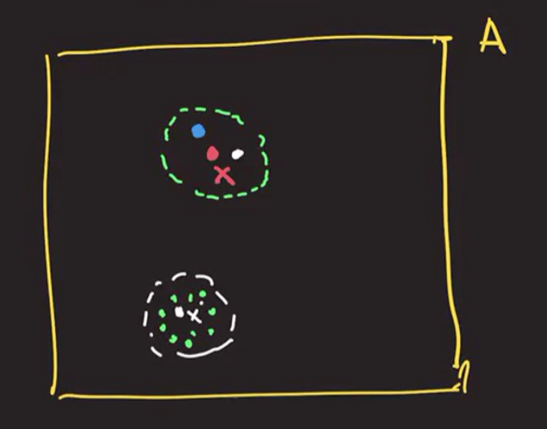
\includegraphics[scale=0.4]{images/2/12}
	\end{center}
	Es decir: 
	$$int(A)=\bigcup_{U\subset A, \  U \text{ es abierto.}} U$$
	i.e $int(A)$ en el abierto más grande contenido. 
	\begin{ejemplo}
		\begin{enumerate}
			\item $int[0,1]=(0,1)$. 
			\item $int \mathbb{R}\cap \mathbb{Z}=\emptyset$. 
			\item $int\mathbb{R}^n=\mathbb{R}^n$.
			\item $A$ es abierto $\iff A=int(A)$. 
		\end{enumerate}
	\end{ejemplo}
\end{definicion}

\begin{ejemplo}
	La cerradura de $A$ es el conjunto: 
	$$\overline{A}:= \bigcap_{A\subset F, \ \text{$F$ cerrado}} F $$
	\begin{nota}
		\begin{enumerate}
			\item $\overline{A}$ es cerrado. 
			\item $\overline{A}$ es el cerrado más pequeño que contiene a $A$. 
			\item $A$ es cerrado $\iff A=\overline{A}$. 
			\item Si $F$ es un cerrado que contiene a $A\implies A\subset \overline{A}\subset F$. 
		\end{enumerate}
	\end{nota}
\end{ejemplo}

\begin{definicion}
	La frontera de $A$ (denotada $bd(A)$ o $\partial A$), se define $$\partial A := \overline{A}-int(A).$$
	\begin{ejemplo}
		Sea $I=[0,1]\implies \overline{I}=[0,1]\implies int(I)=(0,1)\implies \partial A = \overline{I}-int(A)=\{0,1\}$. 
	\end{ejemplo}
\end{definicion}

\begin{definicion}
	El conjunto de todos los puntos de acumulación de un conjunto $A$ se llama conjunto derivada de $A$. Notación: $A'$. 
\end{definicion}

\begin{prop}
	\begin{enumerate}
		\item Si $A\subset B\implies A'\subset B'$. \begin{proof}
			Sea $x\in A'$ (i.e $x$ es un punto de acumulación de $A$) $\implies \ \forall $ abierto $G\ni x\in G$, se tiene que 
			$$(G-\{x\})\cap A\neq \emptyset.$$
			Como $A\subset B\implies (G-\{x\})\cap A\subset (G-\{x\})\cap B\implies \emptyset \neq (G-\{x\})\cap A\subset A \subset (G-\{x\})\cap B\implies (G-\{x\})\cap B\neq \emptyset, \forall G\ni x\in G\implies x\in B'$. 
		\end{proof}
	\item $(A\cup B)'=A'\cup B'$
	\end{enumerate}
\end{prop}